\documentclass[multi, tikz]{article}
\usepackage[utf8]{inputenc}
\usepackage{makecell}

%%%%%%%%%%%%%%%%%%%%%%%% FOREST %%%%%%%%%%%%%%%%%%%%%%%%%
\usepackage{tikz}
\usetikzlibrary{trees}
\usepackage[edges]{forest}
\usepackage{sectsty}
\usepackage{array}
\usepackage{multicol}
\usepackage{graphicx}
\definecolor{folderborder}{RGB}{110,144,169}
\definecolor{folderbg}{rgb}{0.91, 0.84, 0.42}
\usepackage[T1]{fontenc}
\usepackage[utf8]{inputenc} 
\usepackage{floatrow}
\newlength\Size
\setlength\Size{4pt}
\tikzset{%
  folder/.pic={%
    \filldraw [draw=folderborder, top color=folderbg!50, bottom color=folderbg] (-1.05*\Size,0.2\Size+5pt) rectangle ++(.75*\Size,-0.2\Size-5pt);
    \filldraw [draw=folderborder, top color=folderbg!50, bottom color=folderbg] (-1.15*\Size,-\Size) rectangle (1.15*\Size,\Size);
  },
  file/.pic={%
    \filldraw [draw=folderborder, top color=folderborder!5, bottom color=folderborder!10] (-\Size,.4*\Size+5pt) coordinate (a) |- (\Size,-1.2*\Size) coordinate (b) -- ++(0,1.6*\Size) coordinate (c) -- ++(-5pt,5pt) coordinate (d) -- cycle (d) |- (c) ;
  },
}
\forestset{%
  declare autowrapped toks={pic me}{},
  pic dir tree/.style={%
    for tree={%
      folder,
      font=\ttfamily,
      grow'=0,
    },
    before typesetting nodes={%
      for tree={%
        edge label+/.option={pic me},
      },
    },
  },
  pic me set/.code n args=2{%
    \forestset{%
      #1/.style={%
        inner xsep=2\Size,
        pic me={pic {#2}},
      }
    }
  },
  pic me set={directory}{folder},
  pic me set={file}{file},
}
%\newcommand\fname[2]{#1}
\newcommand{\fname}[2]{\begin{tabular}{m{1cm}@{\quad}m{4cm}}#1 & {\color{red}\normalfont#2}\end{tabular}}

\forestset{
  arrow to next tree/.code={
    \draw[dashed] (current bounding box.south east) -- ++(1.5em,0);
    \draw[->](current bounding box.south east) ++(0.25em,0) -- ++(1.5em,0) -- (current bounding box.north east) -- ++(1.5em,0);
  },
  dots below/.style={
    for group={#1}{
      tempdima/.option=y,
      for next node={
        for ancestors={
          TeX={%
            \draw([xshift=\forestregister{folder indent}].parent anchor)--([xshift=\forestregister{folder indent}]\forestoption{x},\forestregister{tempdima}) node[anchor=north]{\vdots};
          },
        },
      },
    },
  },
  prepare fake ancestors/.style={
    for group={#1}{
      init prepare fake parent,
      prepare fake ancestors',
    },
  },
  prepare fake ancestors'/.style={
    if nodewalk valid={parent}{
      for parent={
        prepare fake parent,
        prepare fake ancestors',
      },
    }{},
  },
  init prepare fake parent/.style={
    tempdima/.option=y,
  },
  prepare fake parent/.style={
    y/.register=tempdima, y+=10pt,
    coordinate, edge label={}, no edge,
    tikz={\node at ()[anchor=south,xshift=\forestregister{folder indent}]{\vdots};},
    typeset node,
  },
  draw part of tree/.style 2 args={
    for nodewalk={#1,tempcounta/.option=id}{},
    for nodewalk={#2,tempcountb/.option=id}{},
    draw@part@of@tree/.process=RR{tempcounta}{tempcountb},
  },
  draw@part@of@tree/.style 2 args={
    draw tree processing order/.nodewalk style={
      id=#1,
      ancestors,
      fake={id=#1},
      do until={id()==#2}{next node},
    },
    for root'={
      post draw tree hook/.style={},
      for id={#2}{
        if nodewalk valid={next node}{
          post draw tree hook/.append style={
            to be continued={id=#1}{id=#2},
          },
        }{}
      },
      prepare fake ancestors={id=#1},
      draw tree,
    },
  },
  declare count register=current first node,
  draw linear split tree/.style={
    draw tree method/.append style={post draw tree hook},
    begin draw/.append code={[baseline=(current bounding box.north)]},
    draw tree stage/.style={},
    for root'={current first node/.option=id},
    before typesetting nodes/.process=Ow{id}{
      draw tree stage/.append style={
        draw part of tree={id/.register=current first node}{root',last leaf},
      },
    },
  },
  split here/.style={
    draw tree stage/.append style/.process=ROw2{current first node}{id}{
      draw part of tree={id=##1}{id=##2,previous node},
    },
    current first node/.option=id,
  },
}


%%%%%%%%%%%%%%%%%%%%%%%%%%%%%%%%%%%%%%%%%%%%%%%%%%%%%%%%%%%

\usepackage[a4paper,
  bindingoffset=0.2in,
  left=1in,
  right=1in,
  top=1in,
  bottom=1in,
  footskip=.25in]{geometry}

\title{
    Titolo Progetto \\
    \large Applicazioni e Servizi Web
}

\author{Nome Autore - 000725342 \{razvanflorian.vasile@studio@unibo.it\}}
\date{01 Gennaio 2020}

\usepackage{natbib}
\usepackage{graphicx}

\begin{document}

\maketitle
\section{Introduction}
Introduzione \citep{adams1995hitchhiker}
\subsection{The need for a GUI}

\section{Requirements}
\subsection{User stories}
\begin{table}[!ht]
    \centering
    \resizebox{1\textwidth}{!}{%
      \begin{tabular}{|l|l|l|l|l|l|l|}
        \hline
        \textbf{ID} & \textbf{Priority} & \textbf{Type} & \textbf{As a $<$type of user$>$} & \textbf{I want to $<$perform some task$>$} & \textbf{So that I can $<$achieve some goal$>$} & \textbf{Final} \\ \hline
        1 & Low & Home Page & First-time visitor & Quickly understand what Docker-UI offers & Decide if the application is relevant to me. & Yes \\ \hline
        2 & Low & Documentation Page & Inexperienced user & User-friendly documentation page & Easily learn what features the website offers. & Yes \\ \hline
        3 & Low & Login/Signup Page & New member & Seamlessly load previous sessions' content & Be satisfied and make decisions based on previous data. & Yes \\ \hline
        4.1 & High & Dashboard Page & Registered user & \makecell{Centralized dashboard to interact with a \\ container’s actions} & Manage created containers during their execution. & No \\ \hline
        4.2 & High & Dashboard Functionality & Docker user & Customize projects maintained by DockerUI & Manipulate docker containers via docker-compose files. & No \\ \hline
        5 & High & Logger's Page & Experienced user & See logging messages within the browser & Easily debug running containers. & Yes \\ \hline
        6 & Medium & Docker Hub & Product owner & Simply distribute Docker UI & Dispense the application quickly to interested users. & Yes \\ \hline
      \end{tabular}%
    }%
    \caption{User stories}
\end{table}%

\subsection{Design tasks}
\begin{table}[!ht]
    \centering
    \resizebox{1\textwidth}{!}{%
      \begin{tabular}{|l|l|l|}
    \hline
        \textbf{ID} & \textbf{Type} & \textbf{Design Steps} \\ \hline
        1 & Home Page &
        \makecell[l]{
          1.1. Display a clear and catchy headline that describes our value proposition.\\
          1.2. Include a captivating hero image or illustration that resonates with our brand.\\
          1.3. Add a login button that guides users to explore further.
        }\\ \hline
        2 & Documentation Page &
        \makecell[l]{
          2.1. Setup and host documentation pages via Github Pages.\\
          2.2. Organize the documentation in an easily understandable format.\\
          2.3. Provide comprehensive information on how the website is organized.
        }
        \\ \hline
        3 & Login/Signup Page &
        \makecell[l]{
          3.1. Offer a clear login form with fields for id and password.\\
          3.2. Offer a clear registration page with fields for id, password and email.\\
          3.3. Allow users to sign up using social media accounts for convenience.\\
          3.4. Provide password recovery options and ensure a secure login process.
        }
             \\ \hline
        4.1 & Dashboard design &
        \makecell[l]{
          4.1.1. Design a clean and organized dashboard layout using Figma TODO\\
          4.1.2. Display account information and settings through intuitive and easy to use icons and widgets.\\
          4.1.3. Ensure easy navigation between different sections or features.\\
        }
          \\ \hline
        4.2 & Dashboard Functionaity &
        \makecell[l]{
          4.2.1. buildAll(path) - Used to build all services given a Docker Compose file.\\
          4.2.2. logs(services, path) uses configServices(path) - Show logs of service(s).\\
          4.2.3. kill(path) - Force stop service containers.\\
          4.2.4. stop(path) - Stop running containers without removing them.\\
          4.2.5. start or restartAll(path) - Restart all services.\\
          4.2.6. upAll(path) - Build, (re)creates, starts, and attaches to containers for all services.\\
          4.2.7. down(path) - Stops containers and removes containers, networks, volumes, and images created by up.
        }
        \\ \hline
        5 & Logger's Page &
        \makecell[l]{
          5.1. Redirect container logging messages to the browser to easily read them.\\
          5.2. Create an intuitive interface that allows users to easily navigate across the available features.\\
          5.3. Decide on the technologies necessary to setup the real time interaction between the client and server.
        }
        \\ \hline
        6 & Docker Hub &
        \makecell[l]{
          6.1. Gain the technical expertise needed to setup a Docker Hub release through existing examples. \\
          6.2. Setup dependent containers that need to be installed along-side Docker-UI.\\
          6.3. Exhaustive tests on multiple machines to ensure that the release works consistently across different OSes.
        }
        \\ \hline
    \end{tabular}
    }%
    \caption{User stories}
\end{table}%



\section{Design}
Design dell'architettura del sistema e delle interfacce utente.

\begin{figure}[h!]
\centering
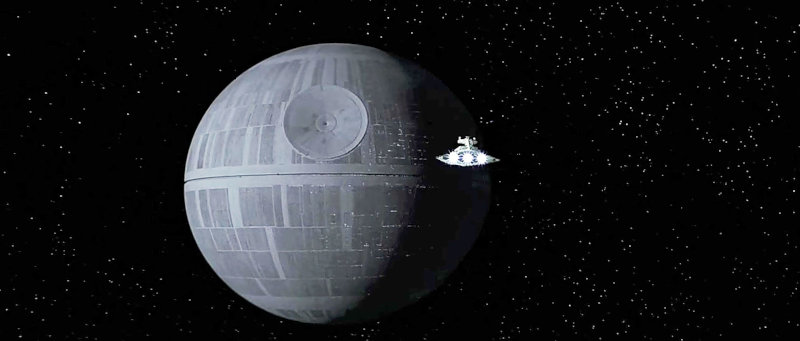
\includegraphics[scale=0.44]{deathStar2.jpg}
\caption{Death Star}
\label{fig:deathstar}
\end{figure}

\section{Technologies}
In terms of dependencies, the requirements that were considered {\em{non
    negotiable}} are MongoDB, ExpressJS, Angular and NodeJS - that is the MEAN
acronym. The extent to which each technology was used will be detailed in the
following section.

Apart from the general requirements imposed by the project guidelines, there
were also used some smaller libraries, of much lesser impact. These libraries
had the role of providing a more fluid and user-friendly browsing experience.


\subsection{The MEAN stack}
Descrizione delle caratteristiche e funzionalità che il sistema prevede.

\subsection{Smaller libraries}
\paragraph{SocketIO}
Used for seamlessly reporting messages while some operation is performed on a
container.

\section{Code}
Solo aspetti rilevanti.
\subsection{Code organization}

\begin{forest}
  pic dir tree,
  where level=0{}{% folder icons by default; override using file for file icons
    directory,
  },
  [server-side
    [bin
      [
        \fname{www.js}{start-up script}, file
      ]
    ],
    [\fname{config}{Env. variables}
      [config.js, file]
    ],
    [controllers
      [container.controller.js, file]
      [user.controller.js, file]
    ]
    [Dockerfile, file]
    [\fname{docker-projects}{}]
    [models
      [container.model.js, file]
      [project.model.js, file]
      [user.model.js, file]
    ]
    [node\_modules]
    [package.json, file]
    [routes
      [container.js, file]
      [user.js, file]
    ]
    [services
      [dockerAdapter.service.js, file]
      [fileSystem.service.js, file]
      [socketIO.service.js, file]
    ]
  ]
\end{forest}

\begin{forest}
  pic dir tree,
  for descendants={% folder icons by default; override using file for file icons
    directory,
  },
  draw linear split tree,
  to be continued/.style 2 args={
    dots below={#2},
    arrow to next tree,
  },
  [client-side
    [\fname{angular.json}{}, file]
    [config
      [\fname{environment.ts}{}, file]
      [\fname{environment.docker.ts}{}, file]
    ]
    [\fname{Dockerfile}{}, file]
    [node\_modules
    ]
    [\fname{package.json}{}, file]
    [\fname{package\_lock.json}{}, file]
    [src
      [\fname{app.component.ts}{}, file]
      [\fname{app.component.html}{}, file]
      [\fname{app.component.css}{}, file]
      [\fname{app.module.ts}{}, file]
      [\fname{app-routing.module.ts}{}, file]
      [base
        [base.module.ts, file]
        [dashboard
          [..., file]
          [\fname{dashboard.module.ts}{}]
        ]
        [footer
          [..., file]
        ]
        [guards
          %[..., file]
        ]
        [models
          %[..., file]
        ]
        [services
          [\fname{operations.service.ts}{}, file]
          [\fname{container.service.ts}{}, file]
          [\fname{socket.service.ts}{}, file]
          [\fname{user.service.ts}{}, file]
        ]
        [toolbar, split here
          %[..., file]
        ]
      ]
      [components
        [dashboard
          [dashboard.module.ts, file]
          [dashboard-routing.module.ts, file]
          [home
            [\fname{...}{testtt}, file]
          ]
          [logger
            [\fname{...}{}, file]
          ]
          [management
            [\fname{...}{}, file]
          ]
          [table
            [\fname{...}{}, file]
          ]
          [table-dialog
            [\fname{...}{}, file]
          ]
        ]
        [user
          [login]
          [register]
          [user.module.ts, file]
          [user-routing.module.ts, file]
        ]
      ]
      [assets
        [icons
          [\fname{...}{}, file]
        ]
      ]
      [\fname{main.ts}{}, file]
      [\fname{styles.scss}{}, file]
    ]
    [\fname{tsconfig.app.json}{}, file]
    [\fname{tsconfig.json}{}, file]
  ]
\end{forest}






\section{Test}
Test effettuati sul codice e test con utenti.

\section{Deployment}
Rilascio, installazione e messa in funzione.
\subsection{Docker deployment}
\begin{figure}[h!]
  \centering
  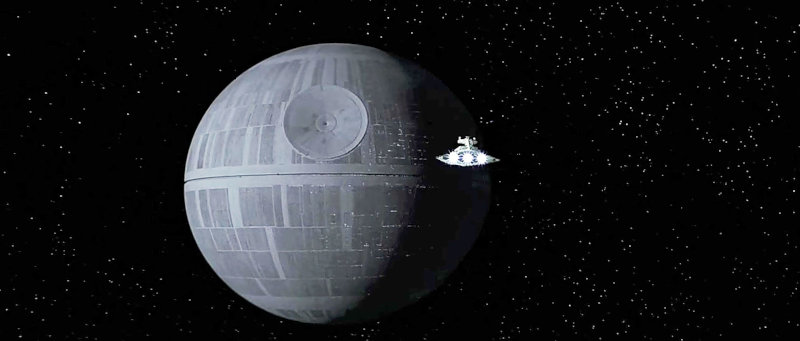
\includegraphics[scale=0.44]{deathStar2.jpg}
  \caption{Docker images}
  \label{fig:deathstar}
\end{figure}

The deployment process was done via Docker. The project used three images for

\section{Conclusion}
Conclusioni

\bibliographystyle{plain}
\bibliography{references}
\end{document}
